\documentclass[border=10pt]{standalone}
\usepackage{pgfplots}
\pgfplotsset{compat=newest}

\begin{document}
		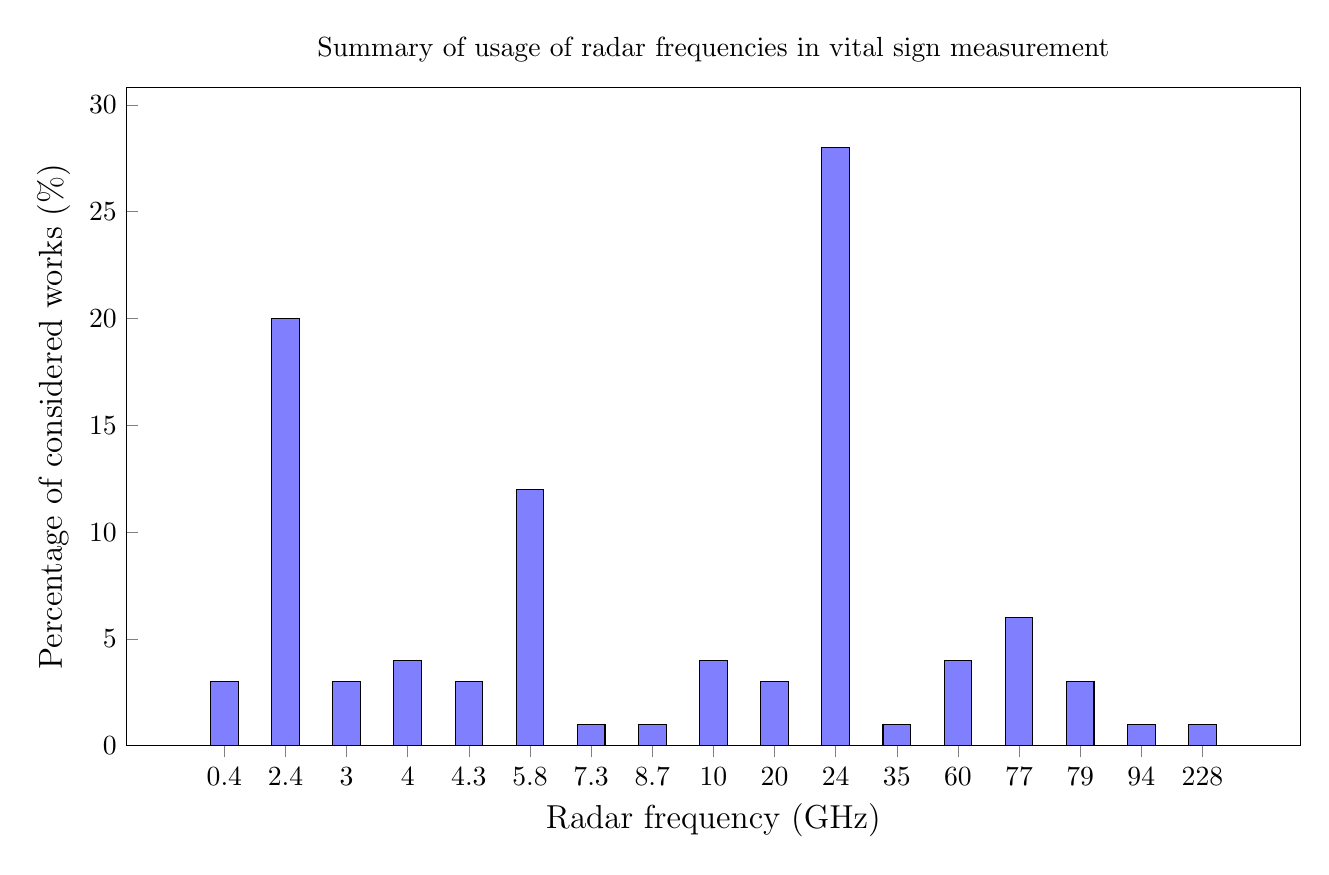
\begin{tikzpicture}
			\begin{axis}[
				title={Summary of usage of radar frequencies in vital sign measurement},
				width=0.95\linewidth,
				ybar,
				ymin=0,
%				axis y line=middle,
%				enlargelimits=0.15,
				xlabel={Radar frequency (GHz)},
				xlabel style={font=\large},
				ylabel={Percentage of considered works (\%)},
				ylabel style={font=\large},				
				xtick=data,
				ytick={0,5,10,15,20,25,30},
				xtick pos=left,
				ytick pos=left,
				% use explicit ticklabels instead of symbolc x coords
				xticklabels={%
					0.4,
					2.4,
					3,
					4,
					4.3,
					5.8,
					7.3,
					8.7,
					10,
					20,
					24,
					35,
					60,
					77,
					79,
					94,
					228,
					},
%				xticklabel style={
%%					  text width=0.1cm,
%%					yshift=-18pt, % move xticks down a bit
%					  align=right,
%					  rotate=90
%				},
%				xlabel style={font=\large},
%				% extra ticks
%				extra x ticks={3,8,13},
%				extra x tick labels={Driving behaviour,Driver Behaviour,Driver Phsiology},
%				extra x tick style={
%					% because the xticklabel style also affects the extra ticks, 
%					% shift extra ticklabels back up
%					ticklabel style={yshift=8.4cm, rotate=-90,align=center,
%					}
%					% tickwidth is actually the length of of the ticks (the small lines)
%%					tickwidth=0
%				},
%				bar width = 5pt,
				x post scale=1.5,
%				height=10cm
				]
				\addplot+[draw=black,fill=blue!50]
				coordinates{
					(1,3)
					(2,20)
					(3,3)
					(4,4)
					(5,3)
					(6,12)
					(7,1)
					(8,1)
					(9,4)
					(10,3)
					(11,28)
					(12,1)
					(13,4)
					(14,6)
					(15,3)
					(16,1)
					(17,1)
				};
%			\legend{DDA,DRA,Both}
			\end{axis}
		\end{tikzpicture}
%
\end{document}